\documentclass[12pt, a4paper]{article}
\usepackage{graphicx}
\usepackage{float}
\usepackage[super, square]{natbib}
\usepackage[margin = 1in]{geometry}
\usepackage{
  color,
  clrscode,
  amssymb,
  ntheorem,
  amsmath,
  listings,
  fontspec,
  xcolor,
  supertabular,
  multirow
}
\definecolor{bgGray}{RGB}{36, 36, 36}
\usepackage[
  colorlinks,
  linkcolor=bgGray,
  anchorcolor=blue,
  citecolor=black
]{hyperref}
\newfontfamily\courier{Courier}

\theoremstyle{margin}
\theorembodyfont{\normalfont}

\newtheorem{theorem}{Theorem}
\newtheorem{definition}[theorem]{Definition}
\newtheorem{example}[theorem]{Example}

\newcommand{\st}{\text{s.t.}}
\newcommand{\mn}{\mathnormal}
\newcommand{\tbf}{\textbf}
\newcommand{\fl}{\mathnormal{fl}}
\newcommand{\f}{\mathnormal{f}}
\newcommand{\g}{\mathnormal{g}}
\newcommand{\R}{\mathbf{R}}
\newcommand{\Q}{\mathbf{Q}}
\newcommand{\JD}{\textbf{D}}
\newcommand{\rd}{\mathrm{d}}
\newcommand{\str}{^*}
\newcommand{\vep}{\varepsilon}
\newcommand{\lhs}{\text{L.H.S}}
\newcommand{\rhs}{\text{R.H.S}}
\newcommand{\con}{\text{Const}}
\newcommand{\oneton}{1,\,2,\,\dots,\,n}
\newcommand{\aoneton}{a_1a_2\dots a_n}
\newcommand{\xoneton}{x_1,\,x_2,\,\dots,\,x_n}


\title{Lecture Notes of Computer Architecture\\\begin{large}(Lecturer \ A-Lei Liang)\end{large}}
\author{Zhou Fan\\ACM Class, Shanghai Jiao Tong University}
\date{}

\begin{document}

\lstset{numbers=left,
  basicstyle=\scriptsize\courier,
  numberstyle=\tiny\courier\color{red!89!green!36!blue!36},
  language=C++,
  breaklines=true,
  keywordstyle=\color{blue!70},commentstyle=\color{red!50!green!50!blue!50},
  morekeywords={},
  stringstyle=\color{purple},
  frame=shadowbox,
  rulesepcolor=\color{red!20!green!20!blue!20}
}
\maketitle
\tableofcontents
\newpage

\section{Pipelining}

  \subsection{Introduction of Pipelining}

	\indent 

	\emph{Pipelining} is an implementation technique whereby multiple instructions are overlapped in execution; it takes advantage of parallelism that exists among the actions needed to execute an instruction.\cite{caqa}

	\subsubsection{Laundry Example}
	  \indent 

	  Suppose we have many loads of clothes to wash, dry and fold. 

	  \begin{itemize}
		\item Each step (washing, drying and folding) is called a \emph{pipe stage} or a \emph{pipe segment}. 
		\item \emph{Latency} is the total time spent on a single task, which is not improved by pipelining.Unbalanced lengths of pipe stages reduces speedup. 
		\item \emph{Throughput} is defined as the number of loads of clothes per minute. It shows how often a load of clothes exits the pipeline.
		\item The time required between moving an instruction one step down the pipeline is a \emph{processor cycle}. In a computer, this processor cycle is usually 1 clock cycle.\cite{caqa}
	  \end{itemize}

	\subsubsection{Speedup from Pipelining}

	  \indent 

	  Throughput is what matters. Pipelining helps \emph{throughput} of whole workload, while it doesn't help \emph{latency} of single task. 

	  \begin{itemize}
		\item Unbalanced lengths of pipe stages reduces speedup. 
		\item Handover time between pipe stages reduces speedup.
	  \end{itemize}

	  To improve the efficiency of a pipeline, one should balance the length of each pipeline stage. If the stages are perfectly balanced, then the time per instruction on the pipeline processor is equal to (under ideal conditions) 
	  $$\frac{\text{Time per instruction on unpipelined machine}}{\text{Number of pipe stages}}$$ 
	  and the throughput of the pipeline is equal to 
	  $$\text{Number of pipe stages} \times \text{Throughput on unpipelined machine}$$

  \subsection{The Basics of a RISC Instruction Set}

	\subsubsection{Introduction of RISC}

	  \indent 

	  A RISC\footnote{reduced instruction set computer} is a computer whose instruction set architecture has lower \emph{cycles per instruction} (CPI) than a CISC\footnote{complex instruction set computer}.

	  MIPS is a RISC instruction set architecture.

	  \paragraph{Key Properties of RISC Architectures\cite{caqa}}
		\begin{itemize}
		  \item All operations on data apply to data in registers and typically change the entire register (32 or 64 bits per register).
		  \item Only load and store operations can affect memory. Load and store operations that load or store less than a full register are often available.
		  \item The instruction formats are few in number, with all instructions typically being one size.
		\end{itemize}

	  These properties make the implementation of pipelining simple.

	  Most RISC architectures like MIPS have three classes of instructions:
	  \begin{enumerate}
		\item ALU\footnote{Arithmetic logic unit} instructions 
		\item Load and store instructions
		\item Branches and jumps
	  \end{enumerate}

	\subsubsection{Implementation of a RISC Instruction Set}

	  \indent

	  The implementation here will focus only on a pipeline for an integer subsetof a RISC architecture that consists of load-store word, branch, and integer ALU operations.

	  \paragraph{Implementation Without Pipelining\cite{caqa}} 
		Every instruction in the RISC subset can be implemented in at most 5 clock cycles as follows:
		\begin{enumerate}
		  \item \emph{Instruction fetch cycle} (IF):

		  Send the program counter (PC) to memory and fetch the current instruction from memory. Update the PC to the next sequential PC by adding 4 (since each instruction is 4 bytes) to the PC\footnote{program counter, indicates where a computer is in its program sequence.}.

		  \item \emph{Instruction decode / register fetch cycle} (ID):

		  Decode the instruction and read the registers corresponding to register source specifiers from the register file. Do the equality test on the registers as they are read, for a possible branch. Sign-extend (introduced later) the offset field of the instruction in case it is needed. Compute the possible branch target address by adding the sign-extended offset to the incremented PC.

		  Decoding is done in parallel with reading registers, which is possible because the register specifiers are at a fixed location in a RISC instruction. This technique is known as \emph{fixed-field decoding}. It may read a register that we don't use, and it doesn't help but also doesn't hurt performance.

		  \item \emph{Execution / effective address cycle} (EX):

		  The ALU operates on the operands prepared in the prior cycle, performing one of three functions depending on the instruction type.
		  \begin{itemize}
			\item Memory reference --- The ALU adds the base register and the offset to form the effective address.
			\item Register-Register ALU instruction --- The ALU performs the operation specified by the ALU opcode on the values read from the register file.
			\item Register-Immediate ALU instruction --- The ALU performs the operation specified by the ALU opcode on the first value read from the register file and the sign-extended immediate.
		  \end{itemize}

		  In a load-store architecture the effective address and execution cycles can be combined into a single clock cycle, since no instruction needs to do both of them.

		  \item \emph{Memory Access} (MEM):

		  The memory does a read using the effective address computed in the previous cycle or writes the data read from the register file using the effective address, if the instruction is a load or a store.

		  \item \emph{Write-back cycle} (WB):

		  For a Register-Register ALU instruction or a load instruction, write the result into the register file.
		\end{enumerate}

	  \paragraph{Sign Extension} In computer arithmetic, sigh extension is the operation of increasing the number of bits of a binary number while preserving the number's sign and value. This is done by appending digits (same as the sign bit) to the most significant side of the number, following a procedure dependent on the particular signed number representation used.
	  
	  For example:
		\begin{itemize}
		  \item ``00 1010'' (decimal positive 10) $\rightarrow$ ``0000 0000 0000 1010''
		  \item ``11 1111 0001'' (decimal negative 15) $\rightarrow$ ``1111 1111 1111 0001''
		\end{itemize}

	  \paragraph{Pipelined Implementation\cite{caqa}}
	  Under ideal conditions, we can easily get a pipelined implementation from the execution described above, doing one of the five steps for five instructions in parallel in each pipeline stage. This procedure is showed in the following table.
	  
	  \begin{table}[H]
	  \centering
	  \begin{tabular}{|l|l|l|l|l|l|l|l|l|l|}
	  \hline
						 & \multicolumn{9}{c|}{Clock Number}               \\ \hline
	  Instruction Number & 1  & 2  & 3  & 4   & 5   & 6   & 7   & 8   & 9  \\ \hline
	  Instruction $i$    & IF & ID & EX & MEM & WB  &     &     &     &    \\ \hline
	  Instruction $i+1$  &    & IF & ID & EX  & MEM & WB  &     &     &    \\ \hline
	  Instruction $i+2$  &    &    & IF & ID  & EX  & MEM & WB  &     &    \\ \hline
	  Instruction $i+3$  &    &    &    & IF  & ID  & EX  & MEM & WB  &    \\ \hline
	  Instruction $i+4$  &    &    &    &     & IF  & ID  & EX  & MEM & WB \\ \hline
	  \end{tabular}
	  \end{table}

  \subsection{Pipeline Hazards}
	\subsubsection{Three Classes of Hazards}

	  Hazards prevent the next instruction in the instruction stream from executing during its designated clock cycle. There are three classes of hazards\cite{caqa}:
	  \begin{enumerate}
		\item \emph{Structural hazards} arise from resource conflicts when the hardware cannot support all possible combinations of instructions simultaneously in overlapped execution.
		\item \emph{Data hazards} arise when an instruction depends on the results of a previous instrucion still in the pipeline.
		\item \emph{Control hazards} is caused by delay between the fetching of instruction and decisions about changes in control flow (branches and jumps).
	  \end{enumerate}

	  These hazards can make it necessary to \emph{stall} the pipeline.

	  There are three generic data hazards\cite{ppt}:
	  \begin{itemize}
		\item Read After Write (RAW):

		$Instr_J$ tries to read oprand before $Instr_I$ writes it.
		\begin{itemize}
		  \item I: add \textbf{r1}, r2, r3
		  \item J: sub r4, \textbf{r1}, r3
		\end{itemize}

		\item Write After Read (WAR):

		$Instr_J$ writes oprand before $Instr_I$ reads it.
		\begin{itemize}
		  \item I: sub r4, \textbf{r1}, r3
		  \item J: add \textbf{r1}, r2, r3
		  \item K: mul r6, r1, r7
		\end{itemize}
		This cannot happen in MIPS 5 stage pipeline.

		\item Write After Write (WAW):

		$Instr_J$ writes oprand before $Instr_I$ writes it.
		\begin{itemize}
		  \item I: sub \textbf{r1}, r4, r3
		  \item J: add \textbf{r1}, r2, r3
		  \item K: mul r6, r1, r7
		\end{itemize}
		This cannot happen in MIPS 5 stage pipeline.

	  \end{itemize}

	\subsubsection{Solutions to Hazards}

	  \paragraph{Forwarding}
	  Some case of data hazards can be avoided using a technique called \emph{forwarding}. Forwarding can be generalized to include passing a result directly to the functional unit that requires it: A result is forwarded from the pipeline register corresponding to the output of one unit to the input of another, or from the result of a unit to the input of the same unit.\cite{caqa}\\
	  However, some data hazards still exists even with forwarding.

	  \paragraph{Software Scheduling}
	  Using software to rearrange instructions is a way to avoid load hazards. In the following example, rearrange instruction order, increase the distance between $Instr_I$ and $Instr_J$ to avoid the hazard:\\
	  \begin{itemize}
		\item I: lw \textbf{r1}, addr
		\item J: add r3, r2, \textbf{r1}
	  \end{itemize}

	  \paragraph{Control Hazards} Alternatives for control hazard\cite{caqa}:
	  \begin{itemize}
		\item Stall until branch direction is clear
		\item Predict Branch Not Taken / Branch Taken
		\item Static Branch Prediction: 
		use profile information collected from ealier runsm, because an individual branch is often highly biased toward taken or untaken.
		\item Dynamic Branch Prediction: 
		predict branches dynamically base on  program behaviour.
	  \end{itemize}

\section{Placeholder}
Sorry for the blank here :-(

To be filled ...

\section{Memory Hierarchy Design}
  \subsection{Memory Technology and Optimizations}
		\subsubsection{Main Memory Organizations}
			THIS PART\cite{ppt}
		  \begin{figure}[H]
				\begin{center}
				  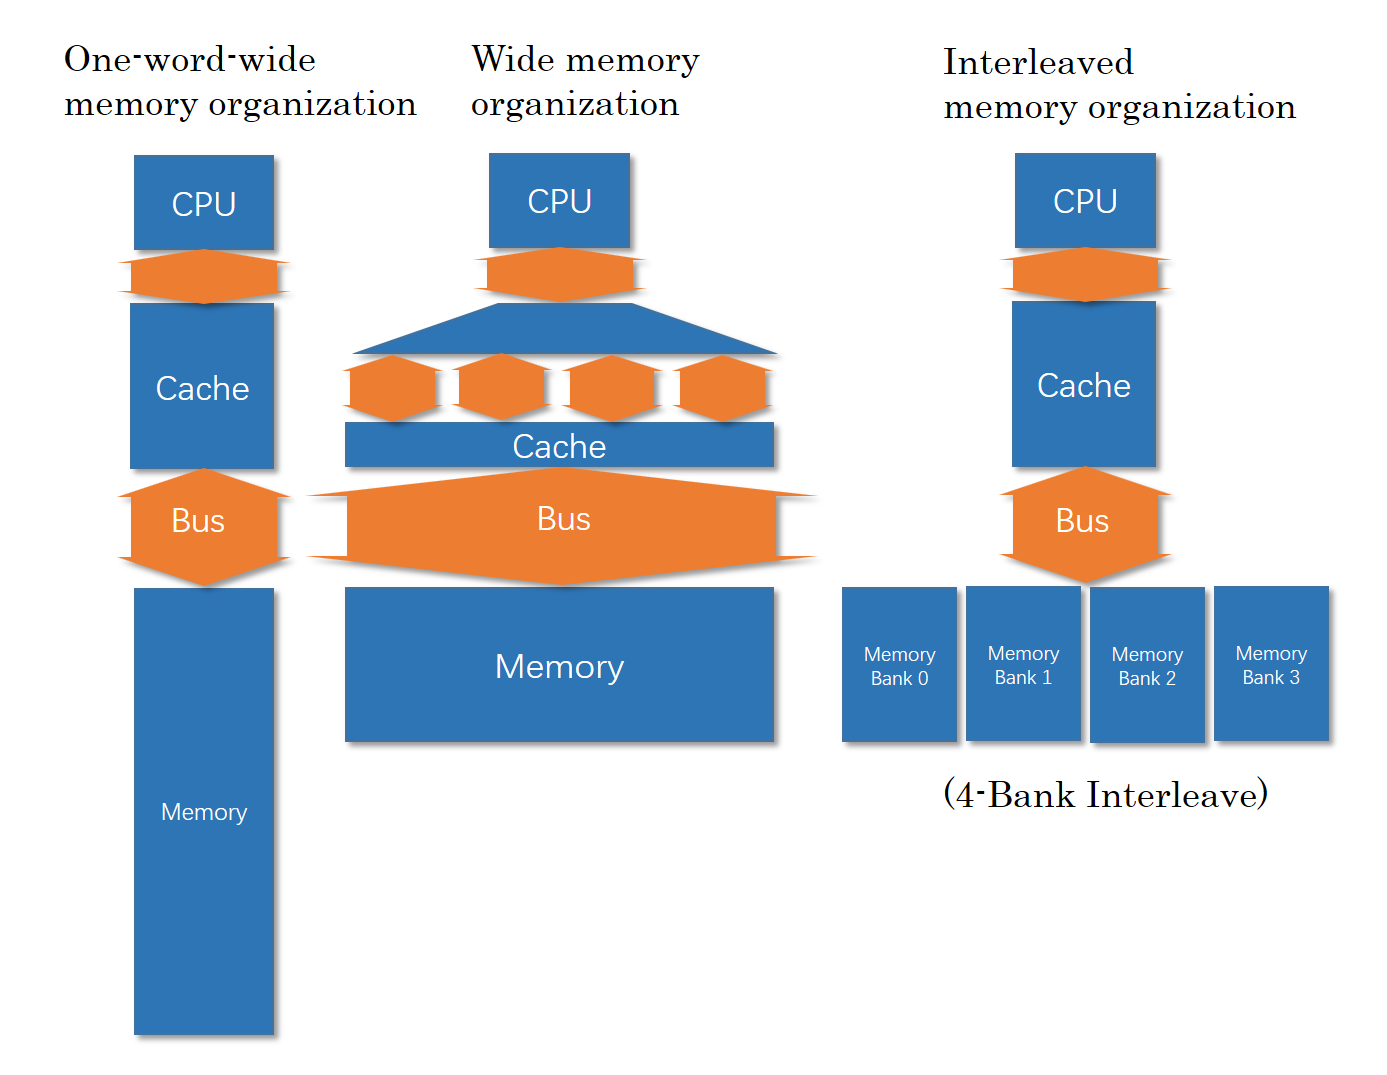
\includegraphics[height=12cm]{images/memory-organizations.png}
				\end{center}
		  \end{figure}
			\begin{itemize}
				\item Simple: CPU, Cache, Bus, Memory same width (32 or 64 bits)
				\item Wide: CPU/Mux 1 word; Mux/Cache, Bus, Memory N words
				\item Interleaved: CPU, Cache, Bus 1 word; Memory N Banks, and these independent memory banks can access data parallelly
			\end{itemize}
			\begin{figure}[H]
				\begin{center}
				  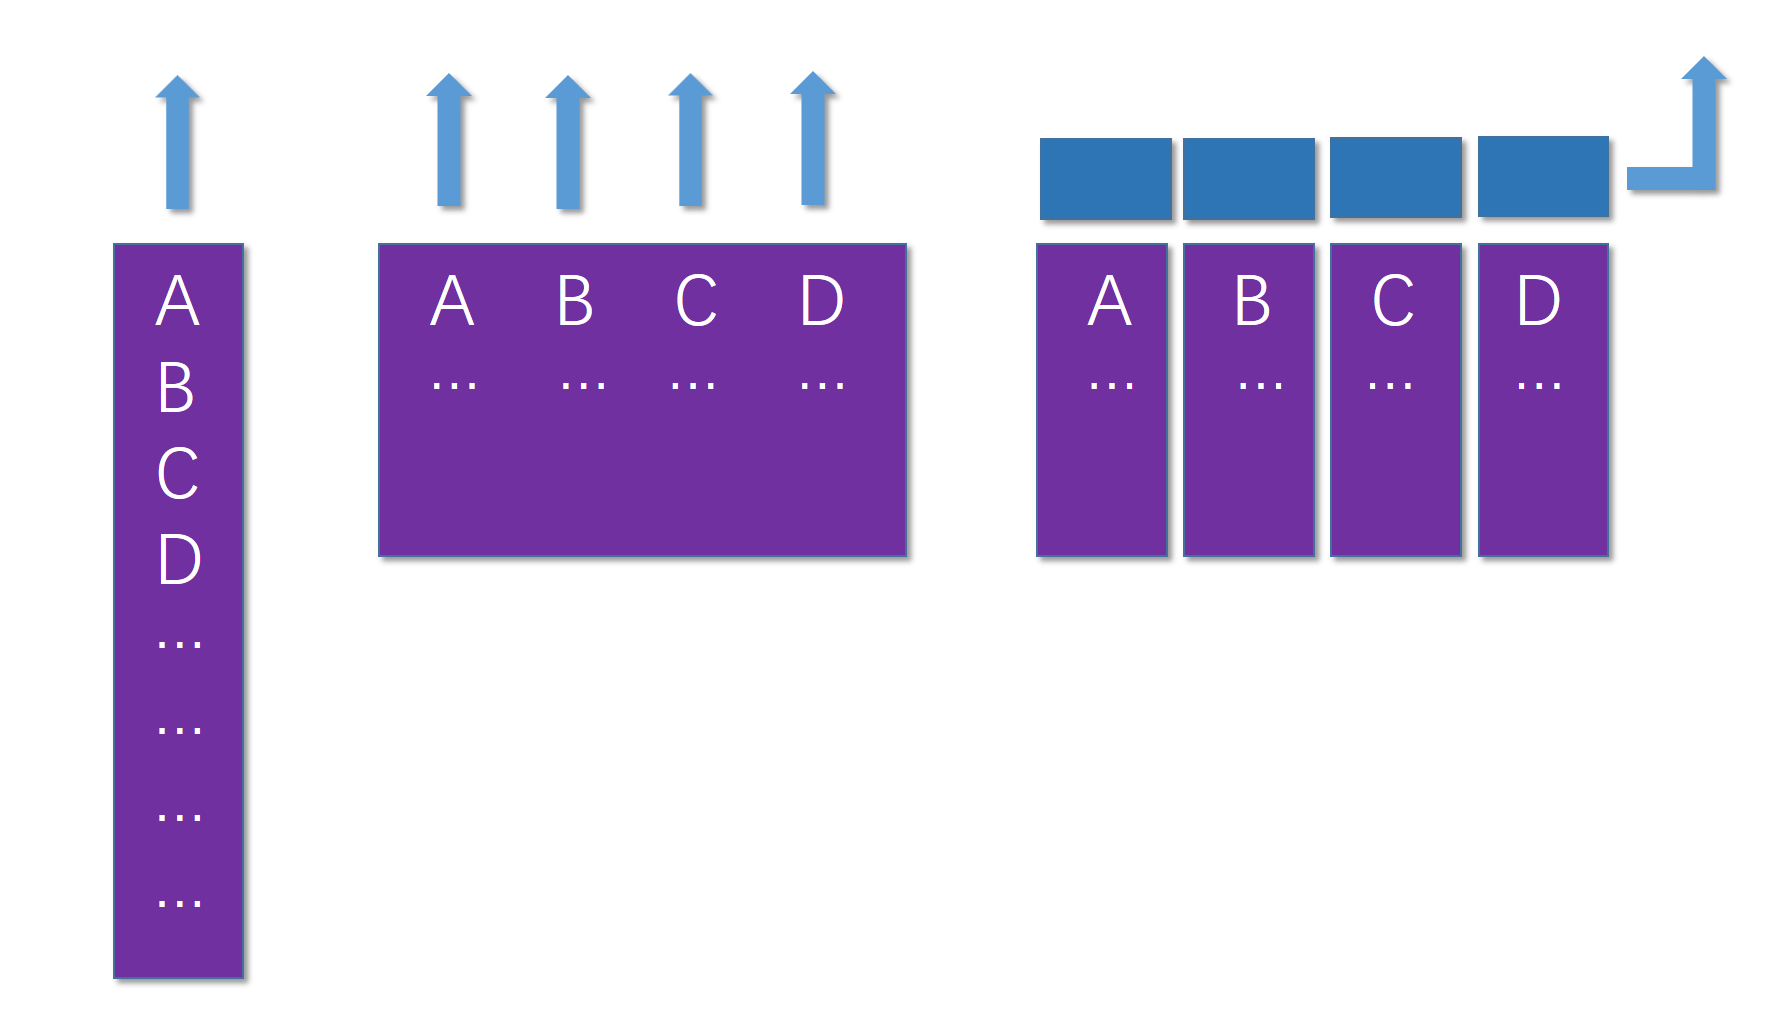
\includegraphics[height=9cm]{images/memory-organization-data.png}
				\end{center}
		  \end{figure}
			\paragraph{Memory Organization Performance}
				Timing model (word size is 32 bits, Cache Block is 4 words):
				\begin{itemize}
					\item 1 to send address
					\item 6 for access time
					\item 1 to send data
				\end{itemize}
				Performance of these three memory organizations under the timing model above:
				\begin{itemize}
					\item Simple: $T=4\times(1+6+1)=32$
					\item Wide: $T=1+6+1=8$
					\item Interleaved: $T=1+6+4\times1=11$
				\end{itemize}
				Wide memory organization has the best time efficiency, but it causes bad compatibility of memory hardwares for its unusual width of Data Bus. Therefore, Interleaved memory organization is often a better choice for PCs.

				\paragraph{Number of Banks} Note that: $\text{number banks} \le \text{number clocks to access word in bank}$, for sequential accesses, otherwise a bank will access a new word before the last accessed one being sent to Bus.

				\paragraph{Avoiding Bank Conflicts} For the following code, independent banks would have no use, for sequential memory accesses come to the same bank since $512\bmod\text{number bank}=0$ if $\text{number bank}=2^k$.
\begin{lstlisting}
int x[256][512];
for (j = 0; j < 512; j = j+1)
    for (i = 0; i < 256; i = i+1)
        x[i][j] = 2 * x[i][j];
\end{lstlisting}
				Solutions to bank conflicts:
				\begin{itemize}
					\item Software: loop interchange or declaring array not power of $2$ ("array padding")
					\item Hardware: prime number of banks
				\end{itemize}
				\begin{figure}[H]
					\begin{center}
					  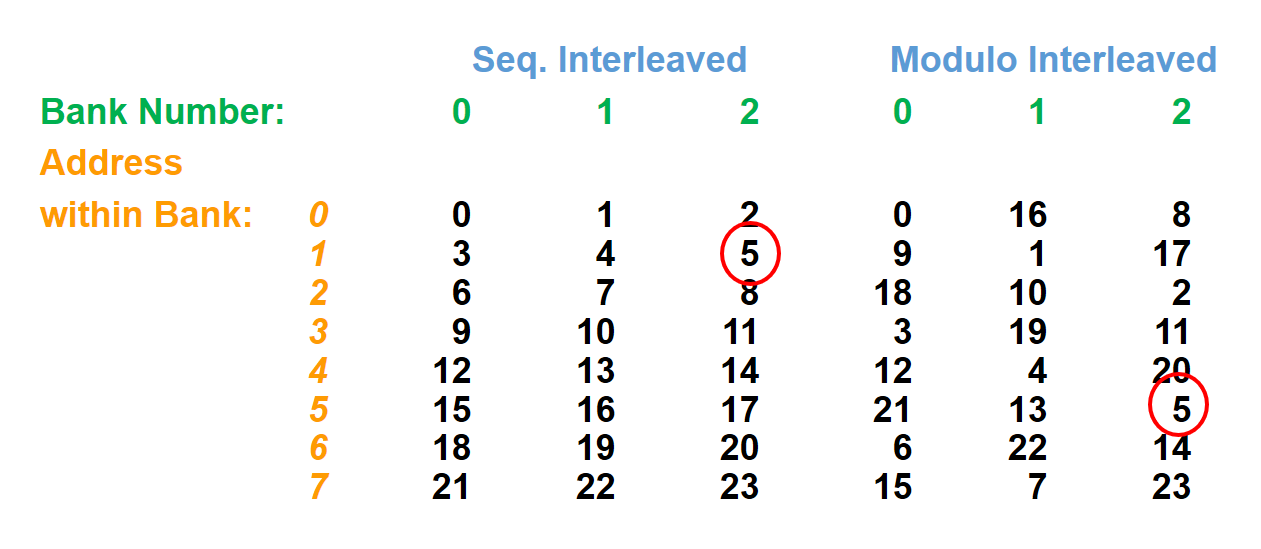
\includegraphics[height=6cm]{images/address-within-bank.png}
					\end{center}
			  \end{figure}
			  \paragraph{Fast Bank Number} Prime number of banks would cause efficiency problem in memory addressing. Assume the address $x$ would be located at $(R_x, C_x)$ of memory. If we set number of banks as a prime $p$,
			  \[R_x = x / p,\ C_x = x \bmod p\]
			  as shown in the \emph{Seq. Interleaved} part of the picture above, and calculation of $x / p$ is pretty time consuming.
				If We arrange data as the \emph{Modulo Interleaved} part of the picture,
				\[R_x = x \bmod 2^k,\ C_x = x \bmod p\]
				and the calculation of $x \bmod 2^k$ is very fast.

				For the calculation of $C_x = x \bmod p$, if we set $p = 2^t - 1$, we have
				\[\begin{split}
				x &= kp + r \\
					&= k(2^t - 1) + r\\
					&= k2^t + r - k \\
				r &\equiv x + k \mod 2^k
				\end{split}\]
				So we can calculate $C_x$ with bit operations, which is very quick.

				And it holds that
				\[(R_i, C_i) \ne (R_j, C_j)\text{ if } i \ne j\]
				It can be proved with the Chinese remainder theorem. So this arrangement of data does work.




\begin{thebibliography}{9}
  \bibitem{caqa} 
	John L. Hennessy, David A. Patterson, et al.
	\emph{Computer Architecture: A Quantitative Approach},
	Fifth Edition, 2012.
  \bibitem{ppt}
	David A. Patterson.
	PPT of \emph{CS252 Graduate Computer Architecture},
	2001
\end{thebibliography}

\end{document}